\documentclass{standalone}
\usepackage{hsbcommon}
\usepackage{pgfplots}
\pgfplotsset{compat=1.18}
\begin{document}
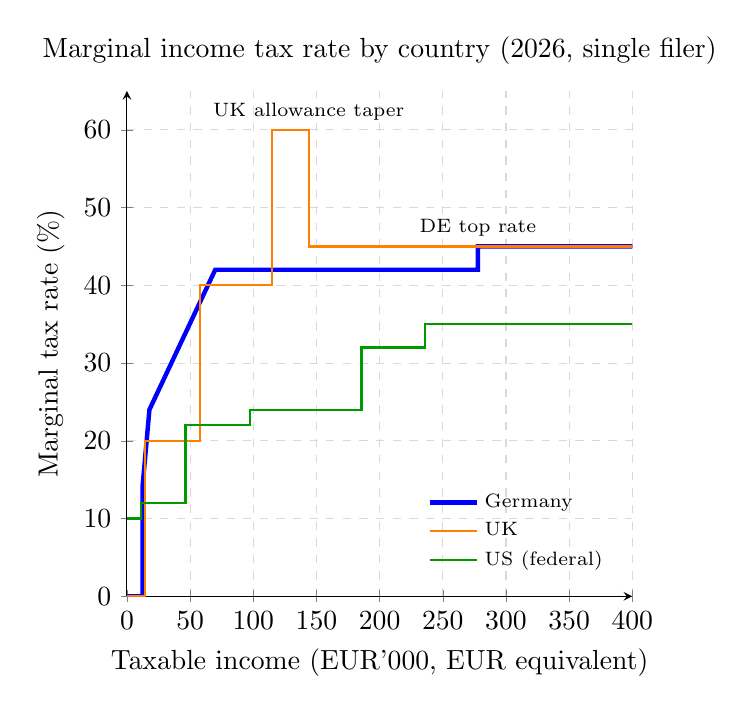
\begin{tikzpicture}
\begin{axis}[
    width=8cm, height=8cm,
    xlabel={Taxable income (EUR{}'000, EUR equivalent)},
    ylabel={Marginal tax rate (\%)},
    xmin=0, xmax=400,
    ymin=0, ymax=65,
    xtick={0,50,100,150,200,250,300,350,400},
    ytick={0,10,20,30,40,50,60},
    grid=major,
    grid style={dashed, gray!30},
    axis lines=left,
    title={Marginal income tax rate by country (2026, single filer)},
    legend pos=south east,
    legend style={font=\scriptsize, draw=none, fill=none},
    legend cell align={left},
]

% Germany
\addplot[ultra thick, color=blue, mark=none] coordinates {
    (0,      0)
    (12.3,   0)
    (12.3,  14)
    (17.8,  24)
    (69.9,  42)
    (277.8, 42)
    (277.8, 45)
    (400,   45)
};
\addlegendentry{Germany}

% United Kingdom
\addplot[thick, color=orange, mark=none] coordinates {
    (0,      0)
    (14.5,   0)
    (14.5,  20)
    (57.8,  20)
    (57.8,  40)
    (115,   40)
    (115,   60)
    (143.9, 60)
    (143.9, 45)
    (400,   45)
};
\addlegendentry{UK}

% United States (federal only), 2026 single, taxable income
% USD thresholds 12,400 / 50,400 / 105,700 / 201,775 / 256,225 / 640,600 at ~0.92 EUR/USD
\addplot[thick, color=green!60!black, mark=none] coordinates {
    (0,     10)
    (11.4,  10)
    (11.4,  12)
    (46.4,  12)
    (46.4,  22)
    (97.2,  22)
    (97.2,  24)
    (185.6, 24)
    (185.6, 32)
    (235.7, 32)
    (235.7, 35)
    (400,   35)
};
\addlegendentry{US (federal)}

% % France
% \addplot[thick, color=purple, mark=none] coordinates {
%     (0,      0)
%     (11.6,   0)
%     (11.6,  11)
%     (29.6,  11)
%     (29.6,  30)
%     (84.6,  30)
%     (84.6,  41)
%     (181.9, 41)
%     (181.9, 45)
%     (400,   45)
% };
% \addlegendentry{France}

% % Sweden
% \addplot[thick, color=red, mark=none] coordinates {
%     (0,      32)
%     (55.3,   32)
%     (55.3,   52)
%     (400,    52)
% };
% \addlegendentry{Sweden}

\node[above] at (axis cs:143.9,60) {\scriptsize UK allowance taper};
\node[above] at (axis cs:277.8,45) {\scriptsize DE top rate};
% \node[below] at (axis cs:55.3,32) {\scriptsize SE state tax kicks in};

\end{axis}
\end{tikzpicture}
\end{document}